\documentclass[10pt]{article}

\usepackage{amsfonts,amsmath,amssymb,amsthm,amsthm}
\usepackage[english]{babel}
\usepackage{microtype}
\usepackage{hyperref}
\usepackage{cleveref}
\usepackage[affil-it]{authblk}
\usepackage{fullpage}
\usepackage{graphicx}

\hfuzz=4pt

\DisableLigatures{encoding = *, family = * }

\newcommand{\norm}[2]{{\left\|#1\right\|}_{#2}}
\newcommand{\ccs}{c_{1,s}}
\newcommand{\ffl}[2]{(-d_x^{\,2})^{#1}#2}
\newcommand{\kernel}[1]{|x-y|^{#1}}
\newcommand{\ue}[1]{#1^{\,\varepsilon}}
\newcommand{\RR}{\mathbb{R}}
\newcommand{\PP}{\mathcal{P}}
\newcommand{\uin}{u_{\textrm{\small in}}}

\makeatletter
\let\@fnsymbol\@arabic
\makeatother

\title{{WKB expansion for a fractional Schrödinger equation}}

\author{Umberto Biccari} 
\affil{\small DeustoTech, University of Deusto, 48007 Bilbao, Basque Country, Spain.}
\affil{Facultad Ingenier\'{\i}a, Universidad de Deusto, Avda Universidades 24, 48007 Bilbao, Basque Country, Spain. \\ Email: \texttt{umberto.biccari@deusto.es}}

\author{Alejandro B. Aceves}
\affil{\small Southern Methodist University, Dedman College of Humanities and Sciences, PO Box 750235, Dallas, Texas, U.S. \\ Email: \texttt{aaceves@smu.edu}}

\date{}

\begin{document}
	
\bibliographystyle{acm}
	
\maketitle 

In recent years, the study of fractional integro-differential equations applied to physics and other areas has faced an extensive growth. In this framework, in the early 2000 Laskin started considering extensions of the classical quantum mechanics theory, based on the idea of replacing the classical Brownian trajectories in Feynman path integrals by Levy flights, which are generated by fractional Laplacians (\cite{laskin2000quantum,laskin2000fractional,laskin2002fractional}). This gave birth to Fractional Quantum Mechanics (FQM), which is the theory of quantum mechanics based on the fractional Schr\"odinger equation (FSE), instead than on the classical integer one. 
 
Later on, these kind of models found applications in several branches of physics, such as the study of condensed-matter realizations of L\'evy cristals (\cite{stickler2013potential}), lasers implementation (\cite{longhi2015fractional}), acoustic wave equations (\cite{liu2009recovery,tanushev2008superpositions}), gravity waves (\cite{tanushev2007mountain}), geophysics (\cite{vcerveny1982computation,hill2001prestack}).

The prototypical example of a fractional Schr\"odinger equation is given by the following one-dimensional non-local partial differential equation
\begin{align}\label{main_eq}
	\PP_s u:= \left[i\partial_t + \ffl{s}{}\right]u = 0, &\;\;  (x,t)\in\RR\times(0,+\infty), 
\end{align}
in which $\ffl{s}{}$ is the fractional Laplacian, defined for all $s\in(0,1)$ and for any function $f$ sufficiently smooth as the following singular integral
\begin{align*}
\ffl{s}{f}(x):=\ccs\; P.V. \int_{\RR}\frac{f(x)-f(y)}{\kernel{1+2s}}\,dy,
\end{align*}
with $\ccs$ a normalization constant given by 
\begin{align*}
	\ccs:= \left(\int_{\RR} \frac{1-\cos(z)}{|z|^{1+2s}}\,dz\right)^{-1} = \frac{s2^{2s}\Gamma\left(s+\frac 12\right)}{\sqrt{\pi}\Gamma(1-s)},
\end{align*}
where $\Gamma$ is the usual Gamma function. 

In \cite{biccari2018wkb}, we developed a study of the propagation properties of the solutions of \eqref{main_eq}, based on a WKB analysis of the equation starting from a highly oscillatory initial datum in the form
\begin{align}\label{in_dat}
	u(x,0) = \uin(x) e^{i\frac{\xi_0}{\varepsilon} x}:=u_0(x),\;\;\; \xi_0\in\RR.
\end{align}

Here, the parameter $\varepsilon$ represents the fast space and time scale introduced in the equation, as well as the typical wavelength of oscillations of the initial datum. 

Asymptotic analysis for wave-like equations through geometric optics (also known as the Wentzel-Kramers-Brillouin (WKB) method or ray-tracing, \cite{brillouin1926mecanique,kramers1926wellenmechanik,spigler1997survey,wentzel1926verallgemeinerung}) is nowadays a classical tool that has been developed in several directions. An incomplete biography on the topic includes \cite{liu2010recovery,liu2013error,liu2015sobolev}. It is by now well-known that wave-type equations, in a local framework, have solutions that are localized near curves $(t,x(t))$ in space-time, also called rays. These curves are, in the interior of the domain of definition of the equation, solutions of a Hamiltonian system of ordinary differential equations which involves the coefficients of the operator. When one of these trajectories hits the boundary of the domain it is reflected according to the classical laws of optics.

In the case of equation \eqref{main_eq}, since $\PP_s=i\partial_t+\ffl{s}{}$ is a pseudo-differential operator with principal symbol $p_s(x,t,\xi,\tau) = \tau - |\xi|^{2s}$, the Hamiltonian system is given by
\begin{align*}
	\begin{cases}
		\dot{x}(\sigma) = \partial_\xi p_s = \pm 2s|\xi(\sigma)|^{2s-1}, & x(0)=x_0
		\\
		\dot{t}(\sigma) = \partial_\tau p_s = 1, & t(0)=0
		\\
		\dot{\xi}(\sigma) = -\partial_x p_s = 0, & \xi(0)=\xi_0
		\\
		\dot{\tau}(\sigma) = -\partial_t p_s =0, & \tau(0)=|\xi_0|^{2s}.
	\end{cases}
\end{align*}

In addition, this system can be easily solved explicitly, and we obtain the following expressions for the bicharacteristics
\begin{align*}
	\begin{cases}
		x(\sigma) = x_0 \pm 2s|\xi_0|^{2s-1}\sigma
		\\
		t(\sigma) = \sigma 
		\\
		\xi(\sigma) = \xi_0
		\\
		\tau(\sigma) = |\xi_0|^{2s}.
	\end{cases}
\end{align*}

In particular, the rays of $\PP_s$ are given by the curves $(t,x_0\pm 2s|\xi_0|^{2s-1}t)\in(0,+\infty)\times\RR$. Notice that, as one expects since the operator has constant coefficients, these rays are straight lines.

The approach that we use for building localized solutions is quite standard. In particular, we look for quasi-solutions to \eqref{main_eq} introducing the ansatz  
\begin{align}\label{ansatz}
	\ue{u}(x,t) = \varepsilon^s e^{i\left[\xi_0\varepsilon^{-1}x\,+\,|\xi_0|^{2s}\varepsilon^{-2s}t\right]}\sum_{j\geq 0}\varepsilon^{\frac{s}{2}j}a_j\left(x,\varepsilon^{\frac{3}{2}s}t\right),
\end{align}
where the normalization constant $\varepsilon^s$ is chosen asking that the function $\ue{u}$ has $H^s(\RR)$-norm of the order $\mathcal O(1)$. The identification of the $a_j$-s is then carried out imposing
\begin{align*}
\PP_s\ue{u} = O(\varepsilon^{\infty}), 
\end{align*} 
thus obtaining a series of PDEs in which it is possible to clearly separate the leading order terms, with respect to $\varepsilon$, from several remainders which will vanish as $\varepsilon\to 0$. This generates a cascade system for the functions $a_j$, which can then be determined as the solution of certain given Partial Differential Equations. In our case, the cascade system is the following one
\begin{align}\label{cascade_system}
	\begin{cases}
		i\partial_\tau a_0 + \mathcal{C}_{\frac s2} \mathcal{D}^{\frac{s}{2}} a_0 = 0  
		\\
		i\partial_\tau a_1 + \mathcal{C}_{\frac s2} \mathcal{D}^{\frac{s}{2}} a_1 + \mathcal{C}_{s} \mathcal{D}^{s} a_0 = 0  
		\\
		i\partial_\tau a_2 + \mathcal{C}_{\frac s2} \mathcal{D}^{\frac{s}{2}} a_2 + \mathcal{C}_{s} \mathcal{D}^{s} a_1 + \mathcal{C}_{\frac{3s}{2}} \mathcal{D}^{\frac{3s}{2}} a_0(\theta,\tau) = 0, & \displaystyle x\leq\theta\leq x+\frac{\varepsilon}{\xi_0}q
		\\
		i\partial_\tau a_j + \mathcal{C}_{\frac s2}\mathcal{D}^{\frac{s}{2}}a_j + \mathcal{C}_{s} \mathcal{D}^{s}a_{j-1} + 	\mathcal{C}_{\frac{3s}{2}} \mathcal{D}^{\frac{3s}{2}}a_{j-2}(\theta,\tau) + \ffl{s}{a_{j-3}}, & j\geq 3
		\\
		&\displaystyle x\leq\theta\leq x+\frac{\varepsilon}{\xi_0}q.  
	\end{cases}
\end{align}  
with $\tau:=\varepsilon^{\frac 32 s}t$ and where $\mathcal{D}^{\,\beta}$ denotes the following fractional derivative of order $\beta$
\begin{align*}
	\mathcal{D}^{\beta} f(x):= \frac{1}{\Gamma(1-\beta)}\int_{-\infty}^x \frac{f'(y)}{(x-y)^{\beta}}\,dy.
\end{align*} 

Moreover, \eqref{cascade_system} is uniquely solvable with initial conditions imposed at $\tau = 0$ and this, of course, allows to identify the expressions of the functions $a_j$. See \cite{biccari2018wkb} for more details.

To the best of our knowledge, a WKB approach has not yet been fully developed in a non-local setting, and our work represents a first step in this direction, providing a complete procedure for obtaining a WKB expansion of equation \eqref{main_eq}. 

Our study is motivated by control problems. Indeed, it is by now well-known that geometric optics constructions for wave-like equations can be used for deriving controllability properties. These properties are usually formulated by means of an observability inequality, in which the total energy of the solutions is uniformly estimated by a partial measurement (typically, the portion of energy localized in a subset of the domain or of its boundary). In this framework, the existence of localized solutions gives sharp necessary conditions for the observability property to hold. In fact, as it was remarked by Ralston in \cite{ralston1982gaussian}, in order to observe these solutions the observation set must intersect every ray. If this were not the case, one could construct a quasi solution along a ray that would not hit the observation set and which, being negligible outside an arbitrarily small neighborhood of the ray, could not be observed. This is the so-called Geometric Control Condition (GCC), which has been proved to be almost sufficient by Bardos, Lebeau and Rauch in \cite{bardos1992sharp}, and necessary by Burq and Gérard in \cite{burq1997condition}.

In the particular case under analysis, we are able to show that given a ray $(t,x(t))$ it is possible to construct quasi-solutions of the fractional Schr\"dinger equation such that the amount of their energy outside a ball of radius $\varepsilon^{\frac 14}$ centered at $x(t)$ is of the order of $\varepsilon^{\frac 14}$. In more detail, we can show that if $\uin\in L^2(\RR)$ and $\ue{u}$ is constructed employing the expansion \eqref{ansatz}, then

\begin{enumerate}
	\item The functions $\ue{u}$ are approximate solutions to \eqref{main_eq}: on the one hand, we have that the function $\ue{z}$ a time $t=0$ is close, in the $L^2$-norm, to any initial datum in the form \eqref{in_dat}
	\begin{align*}
		\norm{u_0(x)-\ue{u}(x,0)}{L^2(\RR)} = \mathcal{O}(\varepsilon^{\frac{1}{2}}),\;\;\;\forall\varepsilon>0.
	\end{align*}
	On the other hand, the same remains true also for any other time $t>0$.
	\begin{align*}
		\norm{u(x,t)-\ue{u}(x,t)}{L^2(\RR)} = \mathcal{O}(\varepsilon^{\frac 12}),\;\;\;\forall\varepsilon>0.
	\end{align*}
	Hence, the functions $\ue{z}$ are really approximating the real solution of \eqref{main_eq} in a $L^2$-setting.
	\item The initial energy of $\ue{z}$, i.e. the energy at $t=0$, is essentially bounded, up to some small reminder which vanishes as $\varepsilon\to 0^+$: 
	\begin{align*}
		\norm{\ue{u}(x,0)}{H^s(\RR)}^2 \approx 1.
	\end{align*}
	Also in this case, as a consequence of the energy conservation property, this same fact remains true for all times $t>0$. 
	\item The amount of energy away from a given ray $(t,x(t))$ of size $\varepsilon^{\frac 14}$ is of the same order $\varepsilon^{\frac 14}$:
	\begin{align*}
		\int_{|x-x(t)|>\varepsilon^{\frac 14}} \left|\ffl{\frac s2}{\ue{u}}(x,t)\right|^2\,dx = \mathcal O(\varepsilon^{\frac 14}).
	\end{align*}	
	In other words, the energy which is not concentrated along $x(t)$ is negligible with respect to the total amount. This third property is possibly the most important one, since it justify the possibility to analyze the propagation of the solutions of \eqref{main_eq} simply in terms of the propagation of the rays. 
\end{enumerate}

In order to study propagation properties of the solutions of our equation in terms of the propagation of the rays, a very important quantity that we shall consider is the so-called \textit{group velocity}, which can be easily computed as 
\begin{align*}
	v=\left|\frac xt\right| = 2s\varepsilon^{1-2s}|\xi_0|^{2s-1}.
\end{align*}

From the above formula we immediately see that, for $s=1/2$ we have $v=1$, i.e. the velocity is constant and independent of the frequency $\xi_0$. For $s\in(0,1/2)$, instead, we have that $1-2s>0$. Hence, taking $\varepsilon<1$, we easily get
\begin{align*}
	v<|\xi_0|^{2s-1}.
\end{align*}
Finally, for $s\in(1/2,1)$ the situation is the opposite. We have $1-2s<0$ and, for $\varepsilon<1$, 
\begin{align*}
	v>|\xi_0|^{2s-1}.
\end{align*}

Hence, we can conclude that for $s> 1/2$ the group velocity increases with the frequency and that the high frequency solutions are traveling faster and faster. On the other hand, for $s<1/2$, the group velocity decreases with the frequency the high frequency solutions are traveling and slower and slower. This behavior has then consequences from the point of view of observation properties for the solutions and, in particular, it confirms the already known results presented in \cite{biccari2014internal}.

\begin{figure}[h]
	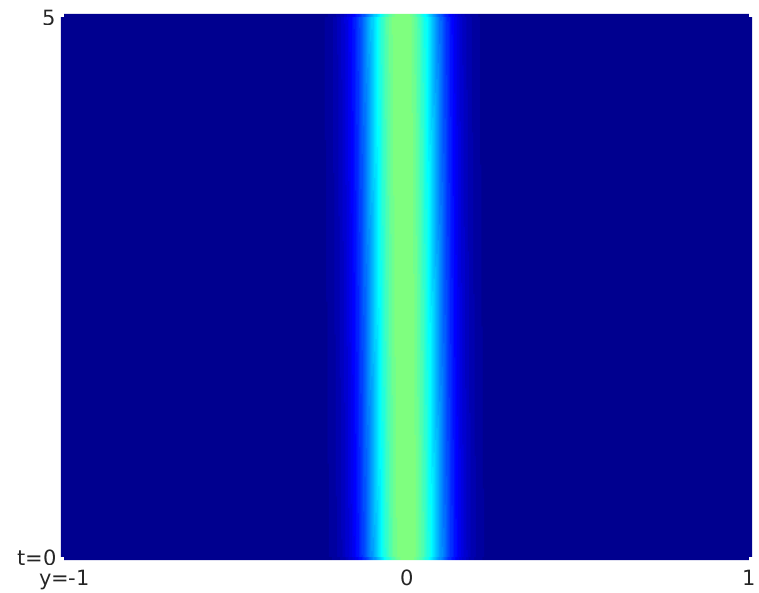
\includegraphics[width=8cm]{../figures-latex/plot_frac_schrodinger1_01_1.png}
\end{figure}

\bibliography{biblio}
\end{document}